\section{The Software Out-of-Order Processor}
\label{sec:soop}

There are two major challenges in implementing an efficient task
scheduler for Legion:
\begin{itemize}
\item  For correctness, Legion must guarantee that every pair of {\em dependent} tasks is executed 
in sequential order.

\item Legion must deal with and, to
  the extent possible, hide the extremely long latencies associated
  with machines that have both distributed memory and many levels of
  memory hierarchy.
\end{itemize}
We use three techniques to deal with these problems:
\begin{itemize}
\item Nested tasks (subtasks) enjoy an isolation property that allows Legion
to avoid comparing all pairs of tasks for dependences.
Specifically, the only tasks that need to be checked for dependences 
are the immediate subtasks of a common
parent task (see Section~\ref{sec:exec}).

\item Legion uses a {\em deferred execution model} that decouples the issuing
of operations from when operations are performed.  Issued operations wait for other operations on
which they are dependent to complete before executing.  For example, Legion may issue a copy
operation to move the results of a task $a$ to the place where a task $b$ will take the copied data as
an argument.  Tasks $a$ and $b$ and the copy can all be issued, but the copy will not start until
task $a$ completes and task $b$ will not start until the copy completes.

\item Legion uses a {\em  software out-of-order processor}, or SOOP, to schedule tasks.  The SOOP 
is distributed and concurrent, and also extracts nested parallelism from subtasks.
\end{itemize}
Legion's SOOP has a five stage pipeline that  decouples the management of resources from actual
task execution.  The five stages are: dependence analysis (Section~\ref{sec:dep}),
distribution (Section~\ref{sec:dist}),
mapping (Section~\ref{sec:map}),
execution (Section~\ref{sec:exec}),
and clean-up (Section~\ref{sec:clean}).
We discuss each in turn.

\usetikzlibrary{calc}
\begin{figure}[t]
  \centering
  \subfigure[mapping of $cnc_0$ task]{
    \label{sfig:mapping_fig:cnc}
    \begin{tikzpicture}[scale=0.8]
      \partitiontree
      \node(cnc_p0)[very thick,draw,fill=white] at (0.45,0.30) {\tiny $cnc_0$};
      \node(cnc_g0)[very thick,draw,fill=white] at (5.45,0.30) {\tiny $cnc_0$};
      \node(def_top)[very thin,draw,fill=white] at (3.3,4.35) {\tiny ~~---~~};
      \draw[very thick] ($ (top.south)!.5!(ptp.center) $) circle (2pt);
      \draw[very thick] ($ (pvsf.north)!.5!(ptf.center) $) circle (2pt);
      \draw[very thick] ($ (pvsf.250)!.5!(ppp.center) $) circle (2pt);
      \draw[very thick] ($ (p0.north)!.5!(pp0.center) $) circle (2pt);
      \draw[very thick] ($ (pvst.north)!.5!(ptt.center) $) circle (2pt);
      \draw[very thick] ($ (pvst.310)!.5!(pgp.center) $) circle (2pt);
      \draw[very thick] ($ (g0.north)!.5!(pg0.center) $) circle (2pt);
      \draw[very thick,->] (def_top) to [bend right=45] (cnc_p0);
      \draw[very thick,->] (def_top) to [bend left=45] (cnc_g0);
    \end{tikzpicture}
  }
  \subfigure[mapping of $dc_0$ task]{
    \label{sfig:mapping_fig:dc}
    \begin{tikzpicture}[scale=0.8]
      \partitiontree
      %\node(cnc_p0)[very thick,draw,fill=white] at (0.45,0.30) {\tiny $\begin{array}{c}\cancel{cnc_0} \\ dc_0\end{array}$};
      \node(dc_p0)[very thick,draw,fill=white] at (0.45,0.30) 
{\tiny
$\begin{array}{@{}c@{}}
\cancel{cnc_0} \\
dc_0
\end{array}$};
      \node(cnc_p1)[very thin,draw,fill=white] at (1.25,0.30) {\tiny $cnc_1$};
      \node(cnc_pn)[very thin,draw,fill=white] at (2.25,0.30) {\tiny $cnc_{n-1}$};
      \node(cnc_g0)[very thin,draw,fill=white] at (5.45,0.30) {\tiny $cnc_0$};
      \node(dc_g0)[very thick,draw,fill=white] at (5.45,0.75) {\tiny $dc_0$};
      \draw[very thick,->] (cnc_g0.west) to [bend left=70] (dc_g0.west);
      \draw[very thick] ($ (cnc_g0.center) - (0.25,0.25) $) -- ++(0.5,0.5);
      \draw[very thick] ($ (cnc_g0.center) - (0.25,-0.25) $) -- ++(0.5,-0.5);
      \node(cnc_g1)[very thin,draw,fill=white] at (6.25,0.30) {\tiny $cnc_1$};
      \node(cnc_gn)[very thin,draw,fill=white] at (7.25,0.30) {\tiny $cnc_{n-1}$};
      \node(def_top)[very thin,draw,fill=white] at (3.3,4.35) {\tiny ~~---~~};
      \draw[very thin] ($ (top.south)!.5!(ptp.center) $) circle (2pt);
      \draw[very thin] ($ (pvsf.north)!.5!(ptf.center) $) circle (2pt);
      \draw[very thin] ($ (pvsf.250)!.5!(ppp.center) $) circle (2pt);
      \draw[very thin] ($ (p0.north)!.5!(pp0.center) $) circle (2pt);
      \draw[very thin] ($ (p1.north)!.5!(pp1.center) $) circle (2pt);
      \draw[very thin] ($ (pn.north)!.5!(ppn.center) $) circle (2pt);
      \draw[very thin] ($ (pvst.north)!.5!(ptt.center) $) circle (2pt);
      \draw[very thin] ($ (pvst.310)!.5!(pgp.center) $) circle (2pt);
      \draw[very thin] ($ (g0.north)!.5!(pg0.center) $) circle (2pt);
      \draw[very thin] ($ (g1.north)!.5!(pg1.center) $) circle (2pt);
      \draw[very thin] ($ (gn.north)!.5!(pgn.center) $) circle (2pt);
    \end{tikzpicture}
  }
  \subfigure[mapping of $volt_0$ task]{
    \label{sfig:mapping_fig:volt}
    \begin{tikzpicture}[scale=0.8]
      \partitiontree
      \node(dc_p0)[very thin,draw,fill=white] at (0.45,0.30) {\tiny $dc_0$};
      \node(dc_p1)[very thin,draw,fill=white] at (1.25,0.30) {\tiny $dc_1$};
      \node(dc_pn)[very thin,draw,fill=white] at (2.25,0.30) {\tiny $dc_{n-1}$};
      \node(dc_g0)[very thin,draw,fill=white] at (5.45,0.30) {\tiny $dc_0$};
      \node(volt_p0)[very thick,draw,fill=white] at (0.45,0.75) {\tiny $volt_0$};
      \draw[very thick,->] (dc_p0.west) to [bend left=70] (volt_p0.west);
      \draw[very thick] ($ (dc_p0.center) - (0.25,0.25) $) -- ++(0.5,0.5);
      \draw[very thick] ($ (dc_p0.center) - (0.25,-0.25) $) -- ++(0.5,-0.5);
      \draw[very thick] ($ (dc_g0.center) - (0.25,0.25) $) -- ++(0.5,0.5);
      \draw[very thick] ($ (dc_g0.center) - (0.25,-0.25) $) -- ++(0.5,-0.5);
      \node(dc_g0)[very thin,draw,fill=white] at (5.45,0.30) {\tiny $dc_0$};
      \node(dc_g1)[very thin,draw,fill=white] at (6.25,0.30) {\tiny $dc_1$};
      \node(dc_gn)[very thin,draw,fill=white] at (7.25,0.30) {\tiny $dc_{n-1}$};
      \draw[very thick] ($ (dc_g0.center) - (0.25,0.25) $) -- ++(0.5,0.5);
      \draw[very thick] ($ (dc_g0.center) - (0.25,-0.25) $) -- ++(0.5,-0.5);
      \draw[very thick] ($ (dc_g1.center) - (0.25,0.25) $) -- ++(0.5,0.5);
      \draw[very thick] ($ (dc_g1.center) - (0.25,-0.25) $) -- ++(0.5,-0.5);
      \draw[very thick] ($ (dc_gn.center) - (0.25,0.25) $) -- ++(0.5,0.5);
      \draw[very thick] ($ (dc_gn.center) - (0.25,-0.25) $) -- ++(0.5,-0.5);
      \node(def_top)[very thin,draw,fill=white] at (3.3,4.35) {\tiny ~~---~~};
      \draw[very thin] ($ (top.south)!.5!(ptp.center) $) circle (2pt);
      \draw[very thin] ($ (pvsf.north)!.5!(ptf.center) $) circle (2pt);
      \draw[very thin] ($ (pvsf.250)!.5!(ppp.center) $) circle (2pt);
      \draw[very thin] ($ (p0.north)!.5!(pp0.center) $) circle (2pt);
      \draw[very thin] ($ (p1.north)!.5!(pp1.center) $) circle (2pt);
      \draw[very thin] ($ (pn.north)!.5!(ppn.center) $) circle (2pt);
      \draw[very thin] ($ (pvst.north)!.5!(ptt.center) $) circle (2pt);
      \draw[very thin] ($ (pvst.310)!.5!(pgp.center) $) circle (2pt);
      \draw[very thin] ($ (g0.north)!.5!(pg0.center) $) circle (2pt);
      \draw[very thin] ($ (g1.north)!.5!(pg1.center) $) circle (2pt);
      \draw[very thin] ($ (gn.north)!.5!(pgn.center) $) circle (2pt);
      \draw[very thick] ($ (g0.north)!.5!(pg0.center) - (0.1,0.1) $) -- ++(0.2,0.2);
      \draw[very thick] ($ (g0.north)!.5!(pg0.center) - (0.1,-0.1) $) -- ++(0.2,-0.2);
      \draw[very thick] ($ (g1.north)!.5!(pg1.center) - (0.1,0.1) $) -- ++(0.2,0.2);
      \draw[very thick] ($ (g1.north)!.5!(pg1.center) - (0.1,-0.1) $) -- ++(0.2,-0.2);
      \draw[very thick] ($ (gn.north)!.5!(pgn.center) - (0.1,0.1) $) -- ++(0.2,0.2);
      \draw[very thick] ($ (gn.north)!.5!(pgn.center) - (0.1,-0.1) $) -- ++(0.2,-0.2);
      \draw[very thick] ($ (pvst.310)!.5!(pgp.center) - (0.1,0.1) $) -- ++(0.2,0.2);
      \draw[very thick] ($ (pvst.310)!.5!(pgp.center) - (0.1,-0.1) $) -- ++(0.2,-0.2);
      \draw[very thick] ($ (pvst.230)!.5!(psp.center) $) circle (2pt);
      \draw[very thick] ($ (s0.north)!.5!(ps0.center) $) circle (2pt);
      \node(def_pvst)[very thick,draw,fill=white] at (5.3,2.75) {\tiny ~~---~~};
      \draw[very thick,->] (dc_g0.north) to [bend right=30] (def_pvst.270);
      \draw[very thick,->] (dc_g1.north) to [bend right=30] (def_pvst.315);
      \draw[very thick,->] (dc_gn.north) to [bend right=30] (def_pvst.0);
      \node(volt_s0)[very thick,draw,fill=white] at (3.2,0.30) {\tiny $volt_0$};
      \draw[very thick,->] (def_pvst.190) to [bend right=40] (volt_s0.130);
    \end{tikzpicture}
  }
  \label{fig:mapping_fig}
  \caption{Mapping of tasks in region tree}
\end{figure}




\subsection{Depedence Analysis}
\label{sec:dep}
{\small
\begin{tabular}{c|cccc}
             & Exclusive & Atomic   & Simultaneous & Relaxed \\
\midrule
Exclusive    & Dep & Dep & Dep & Dep \\ 
Atomic       & Dep & Same & Cont & Cont \\
Simultaneous & Dep & Cont & Same & None \\
Relaxed      & Dep & Cont & None & None \\
\end{tabular}
}

\subsection{Distribution}
\label{sec:dist}

\subsection{Mapping}
\label{sec:map}

\subsection{Execution}
\label{sec:exec}

\begin{figure}
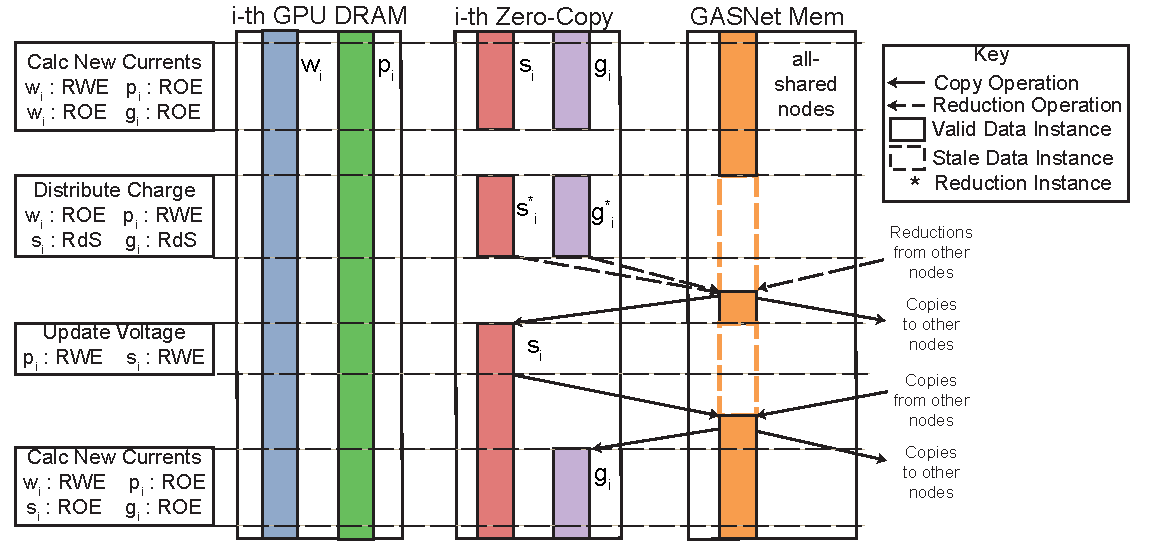
\includegraphics[scale=0.48]{figs/CircuitMem.pdf}
\caption{Tasks and data for the circuit simulation on a cluster of GPUs.}
\end{figure}

\subsection{Clean-Up}
\label{sec:clean}

